%%%%%%%%%%%%%%%%%%%%%%%%%%%%%%%%%%%%%%%%%%%%%%%%%%%%%%%%%%%%%%%%%%%%%%
% LaTeX Template: Curriculum Vitae
%
% Source: http://www.howtotex.com/
% Feel free to distribute this template, but please keep the
% referal to HowToTeX.com.
% Date: July 2011
% 
%%%%%%%%%%%%%%%%%%%%%%%%%%%%%%%%%%%%%%%%%%%%%%%%%%%%%%%%%%%%%%%%%%%%%%
% How to use writeLaTeX: 
%
% You edit the source code here on the left, and the preview on the
% right shows you the result within a few seconds.
%
% Bookmark this page and share the URL with your co-authors. They can
% edit at the same time!
%
% You can upload figures, bibliographies, custom classes and
% styles using the files menu.
%
% If you're new to LaTeX, the wikibook is a great place to start:
% http://en.wikibooks.org/wiki/LaTeX
%
%%%%%%%%%%%%%%%%%%%%%%%%%%%%%%%%%%%%%%%%%%%%%%%%%%%%%%%%%%%%%%%%%%%%%%
\documentclass[paper=a4,fontsize=11pt]{article} % KOMA-article class
							
\usepackage[english]{babel}
\usepackage[utf8x]{inputenc}
\usepackage[protrusion=true,expansion=true]{microtype}
\usepackage{amsmath,amsfonts,amsthm}     % Math packages
\usepackage{graphicx}                    % Enable pdflatex
\usepackage[svgnames]{xcolor}            % Colors by their 'svgnames'
\usepackage{geometry}
%	\textheight=700px                    % Saving trees ;-)
\usepackage{url}

\usepackage[hidelinks]{hyperref}
\usepackage{geometry}
\usepackage{pdfpages}  % Permite adjuntar pdfs al final del documento
\usepackage{wrapfig}
\usepackage{lscape}
\usepackage{rotating}
\usepackage{epstopdf}
\usepackage{textcomp} % hace falta para poner apostrofe
%\usepackage[table]{xcolor} % para las tablas bonitas coloreadas. loads also »colortbl«
\usepackage{array} % necesario para formatear del tiron una columna de una tabla
\usepackage{booktabs}
%\usepackage{pbox} % necesario para introducir salto de linea en celdas de una tabla
\usepackage{longtable}
\usepackage{pdflscape}
\usepackage{amsmath}
\newcommand\T{\textrm{T}}  % "true"
\newcommand\F{\textrm{F}}  % "false"
\usepackage{xspace}
\usepackage{fancyhdr}
 
\pagestyle{fancy}
\fancyhf{}
\lhead{\textbf{Antonio Ortega Jiménez}}
\rhead{\textit{Curriculum Vitae}}
\rfoot{Page \thepage\xspace of 3}

\fancypagestyle{plain}{%
  \fancyhf{}% Clear header/footer
  \fancyfoot[OR]{Page \thepage\xspace of 3}%
  \fancyfoot[EL]{Page \thepage\xspace of 3}%
  \renewcommand{\headrulewidth}{0pt}%
}


\def\changemargin#1#2{\list{}{\rightmargin#2\leftmargin#1}\item[]}
\let\endchangemargin=\endlist  %change the margins as given by arguments



%% Font usage
%%% ------------------------------------------------------------
\usepackage[T1]{fontenc}
\usepackage[osf]{mathpazo}



\frenchspacing              % Better looking spacings after periods
%\pagestyle{empty}           % No pagenumbers/headers/footers


	
%%% Macros
%%% ------------------------------------------------------------
\newlength{\spacebox}
\settowidth{\spacebox}{8888888888}			% Box to align text
\newcommand{\sepspace}{\vspace*{1em}}		% Vertical space macro

\newcommand{\MyName}[1]{ % Name
		\Huge \usefont{OT1}{phv}{b}{n} \hfill #1
		\par \normalsize \normalfont}
		
\newcommand{\MySlogan}[1]{ % Slogan (optional)
		\large \usefont{OT1}{phv}{m}{n}\hfill \textit{#1}
		\par \normalsize \normalfont}

\newcommand{\NewPart}[1]{\section*{
									%\uppercase
									{#1}}}

\newcommand{\PersonalEntry}[2]{
		\noindent\hangindent=2em\hangafter=0 % Indentation
		\parbox{\spacebox}{        % Box to align text
		\textit{#1}}		       % Entry name (birth, address, etc.)
		\hspace{1.5em} #2 \par}    % Entry value

\newcommand{\SkillsEntry}[2]{      % Same as \PersonalEntry
		\noindent\hangindent=2em\hangafter=0 % Indentation
		\parbox{\spacebox}{        % Box to align text
		\textit{#1}}			   % Entry name (birth, address, etc.)
		\hspace{1.5em} #2 \par}    % Entry value	
		
\newcommand{\EducationEntry}[4]{
		\noindent \textbf{#1} \hfill      % Study
		\colorbox{Black}{%
			\parbox{6em}{%
			\hfill\color{White}#2}} \par  % Duration
		\noindent \textit{#3} \par        % School
		\noindent\hangindent=1em\hangafter=0 \small #4 % Description
		\normalsize \par}

\newcommand{\AwardEntry}[4]{
		\noindent \textbf{#1} \hfill      % Study
		\colorbox{Black}{%
			\parbox{3em}{%
			\hfill\color{White}#2}} \par  % Duration
		\noindent \textit{#3} \par        % School
		  \noindent\hangindent=1em\hangafter=0 \small #4  % Description
		\normalsize \par}
		
		
\newcommand{\WorkEntry}[4]{				  % Same as \EducationEntry
		\noindent \textbf{#1} \hfill      % Jobname
		\colorbox{Black}{\color{White}#2} \par  % Duration
		\noindent \textit{#3} \par              % Company
		\noindent\hangindent=2em\hangafter=0 \small #4 % Description
		\normalsize \par}


\newcommand{\VolunteeringEntry}[2]{      % Same as \PersonalEntry
		\noindent\hangindent=2em\hangafter=0 % Indentation
		\parbox{\spacebox}{        % Box to align text
		\textit{#1}}			   % Entry name (birth, address, etc.)
		\hspace{1.5em} #2 \par}    % Entry value	
		
%Shortcuts
\newcommand{\apostrofe}{\textquotesingle\xspace}


%% Custom colors
%%% ------------------------------------------------------------

\usepackage{xcolor}
\definecolor{StrongRed}{RGB}{139,0,0}
\definecolor{DarkRed}{RGB}{200,0,0}
\definecolor{awesome-red}{HTML}{DC3522}
\definecolor{awesome-skyblue}{HTML}{0395DE}
\definecolor{gray}{HTML}{5D5D5D}
\definecolor{lightgray}{HTML}{999999}


%%% Custom sectioning (sectsty package)
%%% ------------------------------------------------------------
\usepackage{sectsty,regexpatch}


\makeatletter

%% Modify the look of the section rule
\newcommand{\setsectionrulecolor}[1]{\colorlet{secrulecolor}{#1}}
\setsectionrulecolor{awesome-red}% default
\xpatchcmd*{\SS@normsectionrule}% <cmd>
  {\rule}% <search>
  {\color{secrulecolor}\rule}% <replace>
  {}{}% <success><failure>
\makeatother

%% Implement the section rule
\sectionfont{%			            % Change font of \section command
	%\usefont{OT1}{phv}{b}{n}%		% bch-b-n: CharterBT-Bold font
	\sectionrule{0pt}{0pt}{-5pt}{1.7pt}} % width of section rule    
	
	
	
%%% Begin Document
%%% ------------------------------------------------------------
\begin{document}
% you can upload a photo and include it here...
%\begin{wrapfigure}{l}{0.5\textwidth}
%	\vspace*{-2em}
%		\includegraphics[width=0.15\textwidth]{photo}
%\end{wrapfigure}

%\MyName{Your Name}
%\MySlogan{Curriculum Vitae}
%
%\sepspace

\thispagestyle{plain}
% Set your name here
\def\name{\textcolor{StrongRed}{Antonio Ortega Jim\'enez}}

\centerline{\LARGE\bf \name}
\vspace{0.1in}
\centerline{\textcolor{awesome-red}{\textsc{Computational Biochemist}}}
\vspace{0.25in}



%%% Personal details
%%% ------------------------------------------------------------
\begin{minipage}[t]{0.6\textwidth}
  \textbf{Citizenship}: Spanish \par
  \textbf{Cell phone}: +34 664 661 687 \par
  \textbf{Email}: \href{mailto:antortjim@alum.us.es}{antortjim@alum.us.es} \par
  \leftskip=1.1cm  \href{mailto:rnq313@alumni.ku.dk}{rnq313@alumni.ku.dk} \par
  \leftskip=0cm \textbf{Website}: \href{http://www.antortega.com}{antortega.com} \par
  
\end{minipage}
\begin{minipage}[t]{0.3\textwidth}
  \textbf{LinkedIn}: \href{http://www.linkedin.com/in/antortjim}{linkedin.com/in/antortjim} \\
   \textbf{SO careers}:\\
   \href{http://careers.stackoverflow.com/antortjim}{careers.stackoverflow.com/antortjim} \\

\end{minipage}

%%% Awards
%%% ------------------------------------------------------------
\NewPart{Awards}{}

\AwardEntry{Best Huelva province high-school record}{2012}{Government of Andalusia}{\begin{changemargin}{0.5cm}{2cm}   
The two best high school students from the province of Huelva were awarded this prize.\end{changemargin}}
\sepspace

\AwardEntry{Paco Anillo Award on Mathematics representing Huelva}{2008}{Andalusian Association for Mathematical Education THALES}{\begin{changemargin}{0cm}{2cm}A prize bestowed in every andalusian province upon the most genuine solution proposed to one of the exercises posed at the Mathematical contest undergone in the same year.\end{changemargin}}

%%% Computational Skills
%%% ------------------------------------------------------------
\NewPart{Computational Skills}

\SkillsEntry{Machine Learning}{Neural Networks, Support Vector Machines, K-means, PCA}
\sepspace

\SkillsEntry{Bioinformatics}{Microarrays, RNA-seq, ChIP-seq, Sequence analysis, Phylogeny,}
\SkillsEntry{}{Modeling, Gene Networks}
\sepspace

\SkillsEntry{Programming languages}{R \& Bioconductor, Octave/MATLAB, Python, HTML, CSS}
\sepspace

\SkillsEntry{Technologies}{Linux, Bash, Vim, Latex, Arduino, GitHub, Inkscape}

%%% Education
%%% ------------------------------------------------------------
\NewPart{Education}{}

\EducationEntry{MSc. Bioinformatics}{2016-2018}{University of Copenhagen}{Prospective student.}
\sepspace

\EducationEntry{BSc. Biochemistry}{2012-2016}{University of Seville}{\textbf{GPA}: 2.57/4.0. \textbf{Average}: 8.43/10 \\
  %\footnote{Computed as $1 + \frac{\mbox{10 based score} - 5}{5} \times 3 $}\\
  Honors on Statistics, Biosynthesis of Macromolecules, Human Genetics, and Bioinformatics.}
 
%%% Projects
%%% ------------------------------------------------------------
\NewPart{Research Projects (wet lab)}{}

\EducationEntry{Characterization of \textit{sigE}\textquotesingle s promoter}{2014-2015}{CIC Cartuja - CSIC}{\begin{changemargin}{0cm}{3cm}Collaborated with Drs. Muro and Vioque's group on the characterization of the \textit{sigE} gene promoter in \textit{Nostoc PCC7120}.\end{changemargin}}

\EducationEntry{Characterization of All1873}{2015-2016}{CIC Cartuja - CSIC}{Carried out my bachelor thesis on the heterologous expression of All1873, a hypothetical protein of unknown function from \textit{Nostoc PCC7120}, in \textit{E. coli}.}
  
  


%%% Conferences attended
%%% ------------------------------------------------------------
\NewPart{Conferences attended}
\VolunteeringEntry{}{}
\VolunteeringEntry{Estudiante}{through simple experimental performances.}


%%% Volunteering
%%% ------------------------------------------------------------
\NewPart{Volunteering}
\VolunteeringEntry{Salón del}{High-school students were encouraged to study the Life Sciences}
\VolunteeringEntry{Estudiante}{through simple experimental performances.}


  


  
  
%%% Online learning
%%% ------------------------------------------------------------
\NewPart{Complementary education}{}


\AwardEntry{Summer School on Bioinformatics}{2015}{Complutense University of Madrid}{}  
  
\AwardEntry{Python Syntax Course}{2015}{Codecademy}{}


\AwardEntry{Machine Learning by Andrew Ng}{2016}{University of Stanford at Coursera}{}


%%% Languages
%%% ------------------------------------------------------------
\NewPart{Languages}

\SkillsEntry{Spanish}{(Mother tongue)}
\sepspace

\SkillsEntry{English}{C1 level (advanced)}
\sepspace

\SkillsEntry{French}{B1 level (basic)}
\sepspace

%\SkillsEntry{Danish}{}



%%%% Work experience
%%%% ------------------------------------------------------------
%\NewPart{Work experience}{}
%
%\EducationEntry{Job name}{2011-present}{Company Name inc., Full-time}{Job description goes here. To maintain a stylish look, try to fill this description with a few lines of text. Do the same for the other entries in this section.}
%\sepspace
%
%\EducationEntry{Job name}{2010-2011}{Company Name inc., Part-time}{Job description goes here. To maintain a stylish look, try to fill this description with a few lines of text. Do the same for the other entries in this section.}


\NewPart{Hobbies}
I enjoy practising sports, particularly jogging and basketball, and I always try to move around Seville by bike. I really enjoy listening to rock and electronic bands like AC/DC and Prodigy. I am fond of learning languages and new cultures. What I love the most is hanging out with my friends and visiting the center of Seville, an astonishingly beautiful city. I was a boy scout until age 11.




\NewPart{Portfolio}

A listing of relevant projects in Bioinformatics carried out during my Bachelor of Science can be retrieved at \href{antortega.com/?p=bioinformatics-portfolio}{antortega.com/?p=bioinformatics-portfolio}.



\NewPart{Appendix}
%\vspace{-0.6cm}
%\textcolor{awesome-red}{\rule{432pt}{0.2pt}} \vspace{-0.0cm}
\begin{enumerate}

%\item \hyperlink{motivation}{Motivation letter} (English)

\item \hyperlink{premio_extraordinario}{Best Huelva province record diploma} (Spanish)
\item \hyperlink{complu}{Summer School on Bioinformatics at Complutense University} (Spanish)

\item \hyperlink{ML-Coursera}{Machine Learning by Andrew Ng Coursera Certificate (English)}

\item \hyperlink{exp-en}{Official college transcript of results} (English)
\item \hyperlink{cae}{Certificate in Advanced English} (English)
\end{enumerate}
%
%\clearpage


% Motivation letter
%\hypertarget{motivation}{}
%\includepdf[pages={1,2}]{carta/Antonio_Ortega_Motivation_Letter.pdf}
%\clearpage


% KU transcript

%\thispagestyle{empty}
\newgeometry{margin=20pt, bottom=5pt}
\hypertarget{KU_transcript}{}
\centering
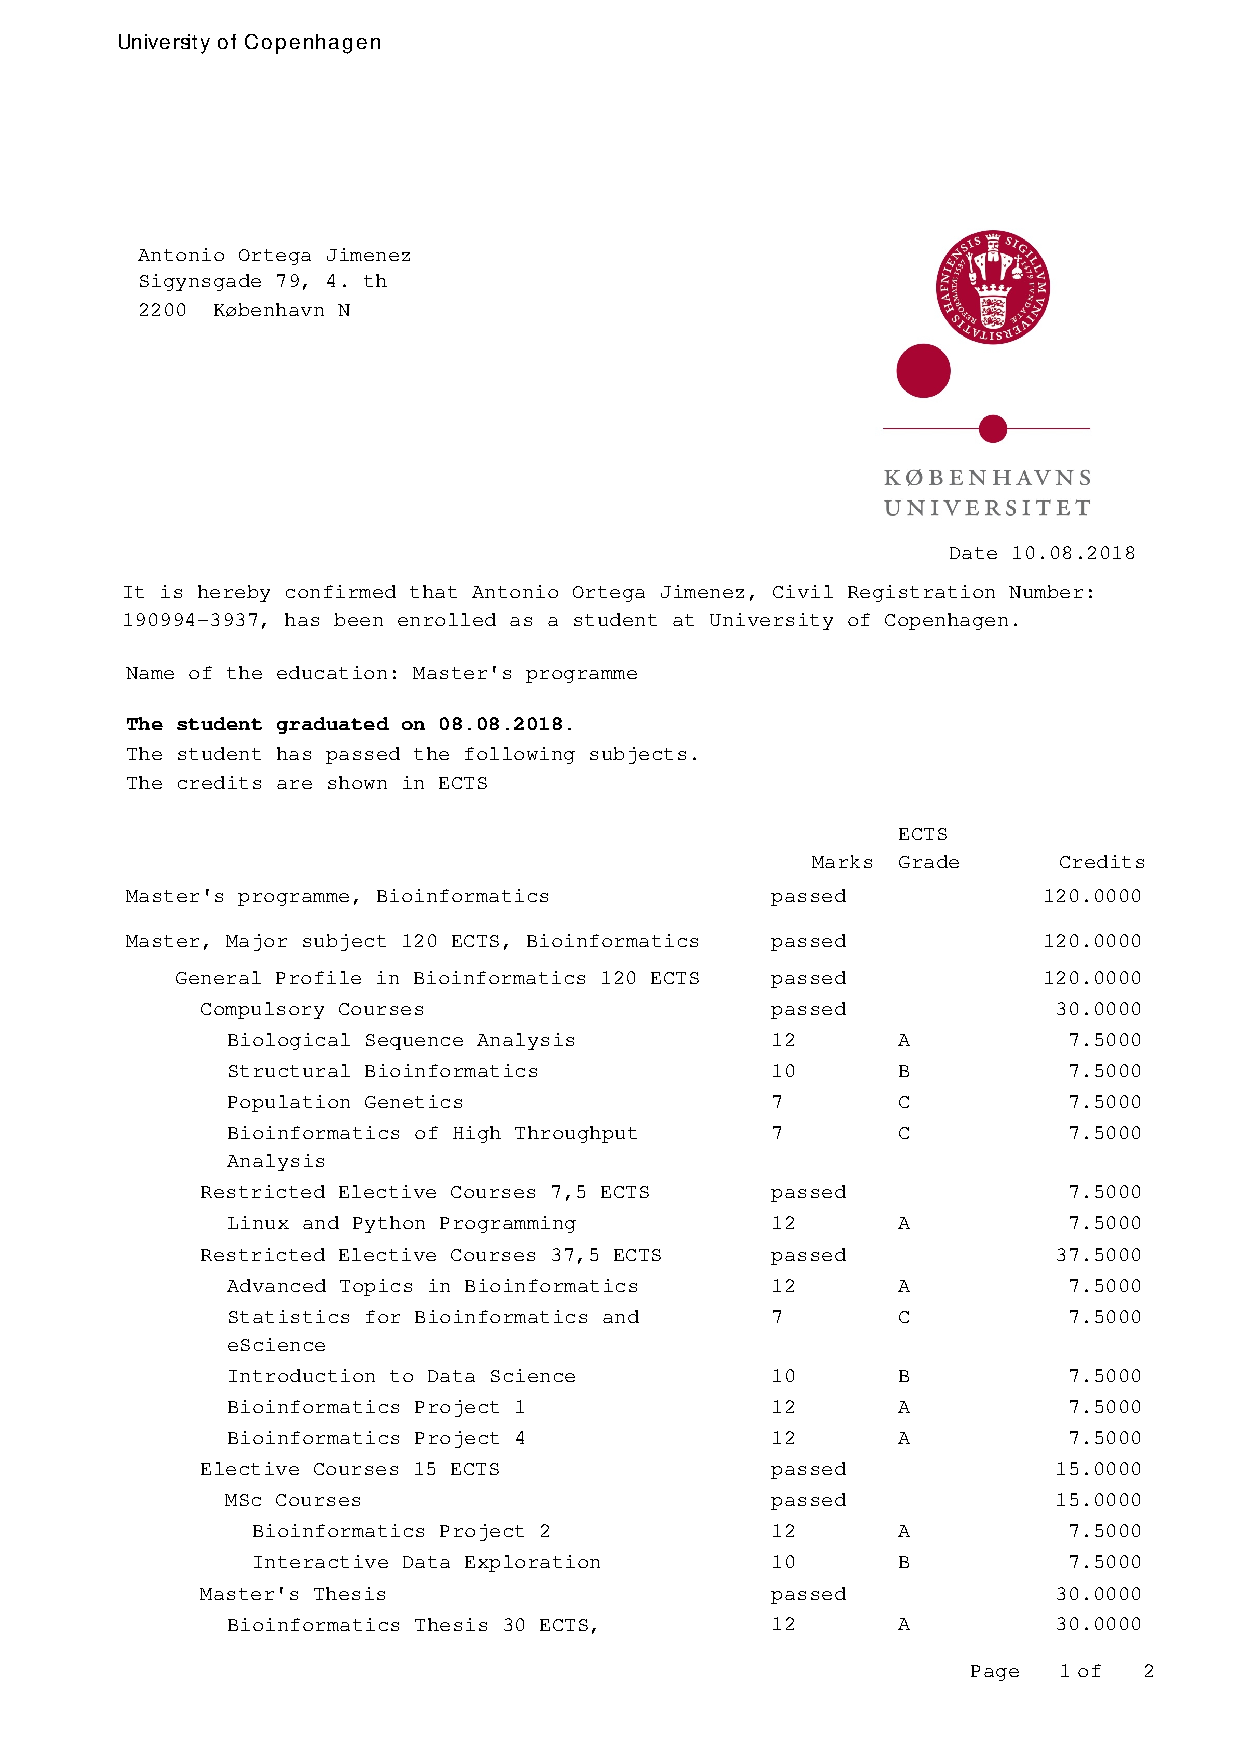
\includegraphics[scale=0.9]{append/transcript.pdf}
\clearpage


%% Diploma del premio extraordinario
%
%%\thispagestyle{empty}
%\newgeometry{margin=20pt, bottom=5pt}
%\hypertarget{premio_extraordinario}{}
%\begin{landscape}
%\centering
%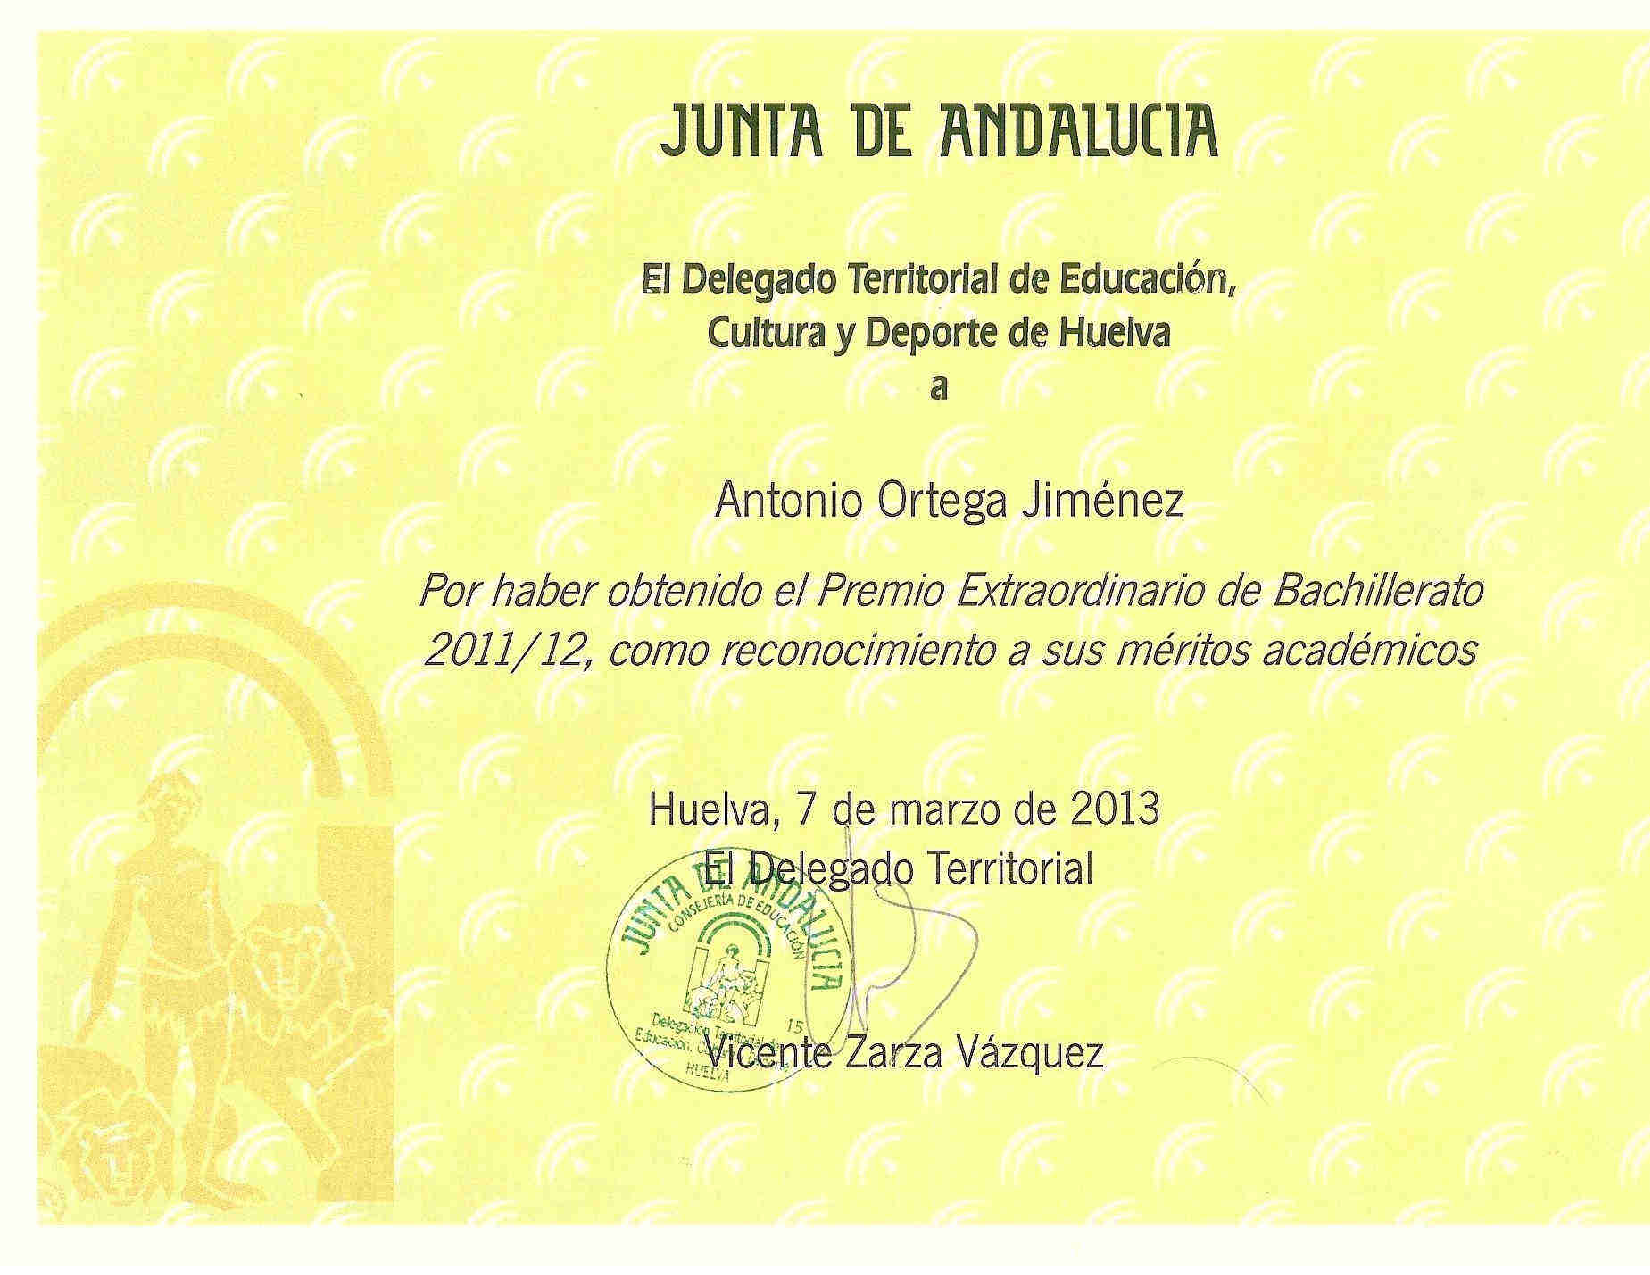
\includegraphics[scale=0.9]{append/premio_extraordinario.pdf}
%\end{landscape}
%\restoregeometry
%\clearpage
%
%
%% Diploma del curso de bioinformatica en la complu
%\thispagestyle{empty}
%
%\newgeometry{margin=20pt, bottom=5pt}
%\hypertarget{complu}{}
%\begin{landscape}
%\centering
%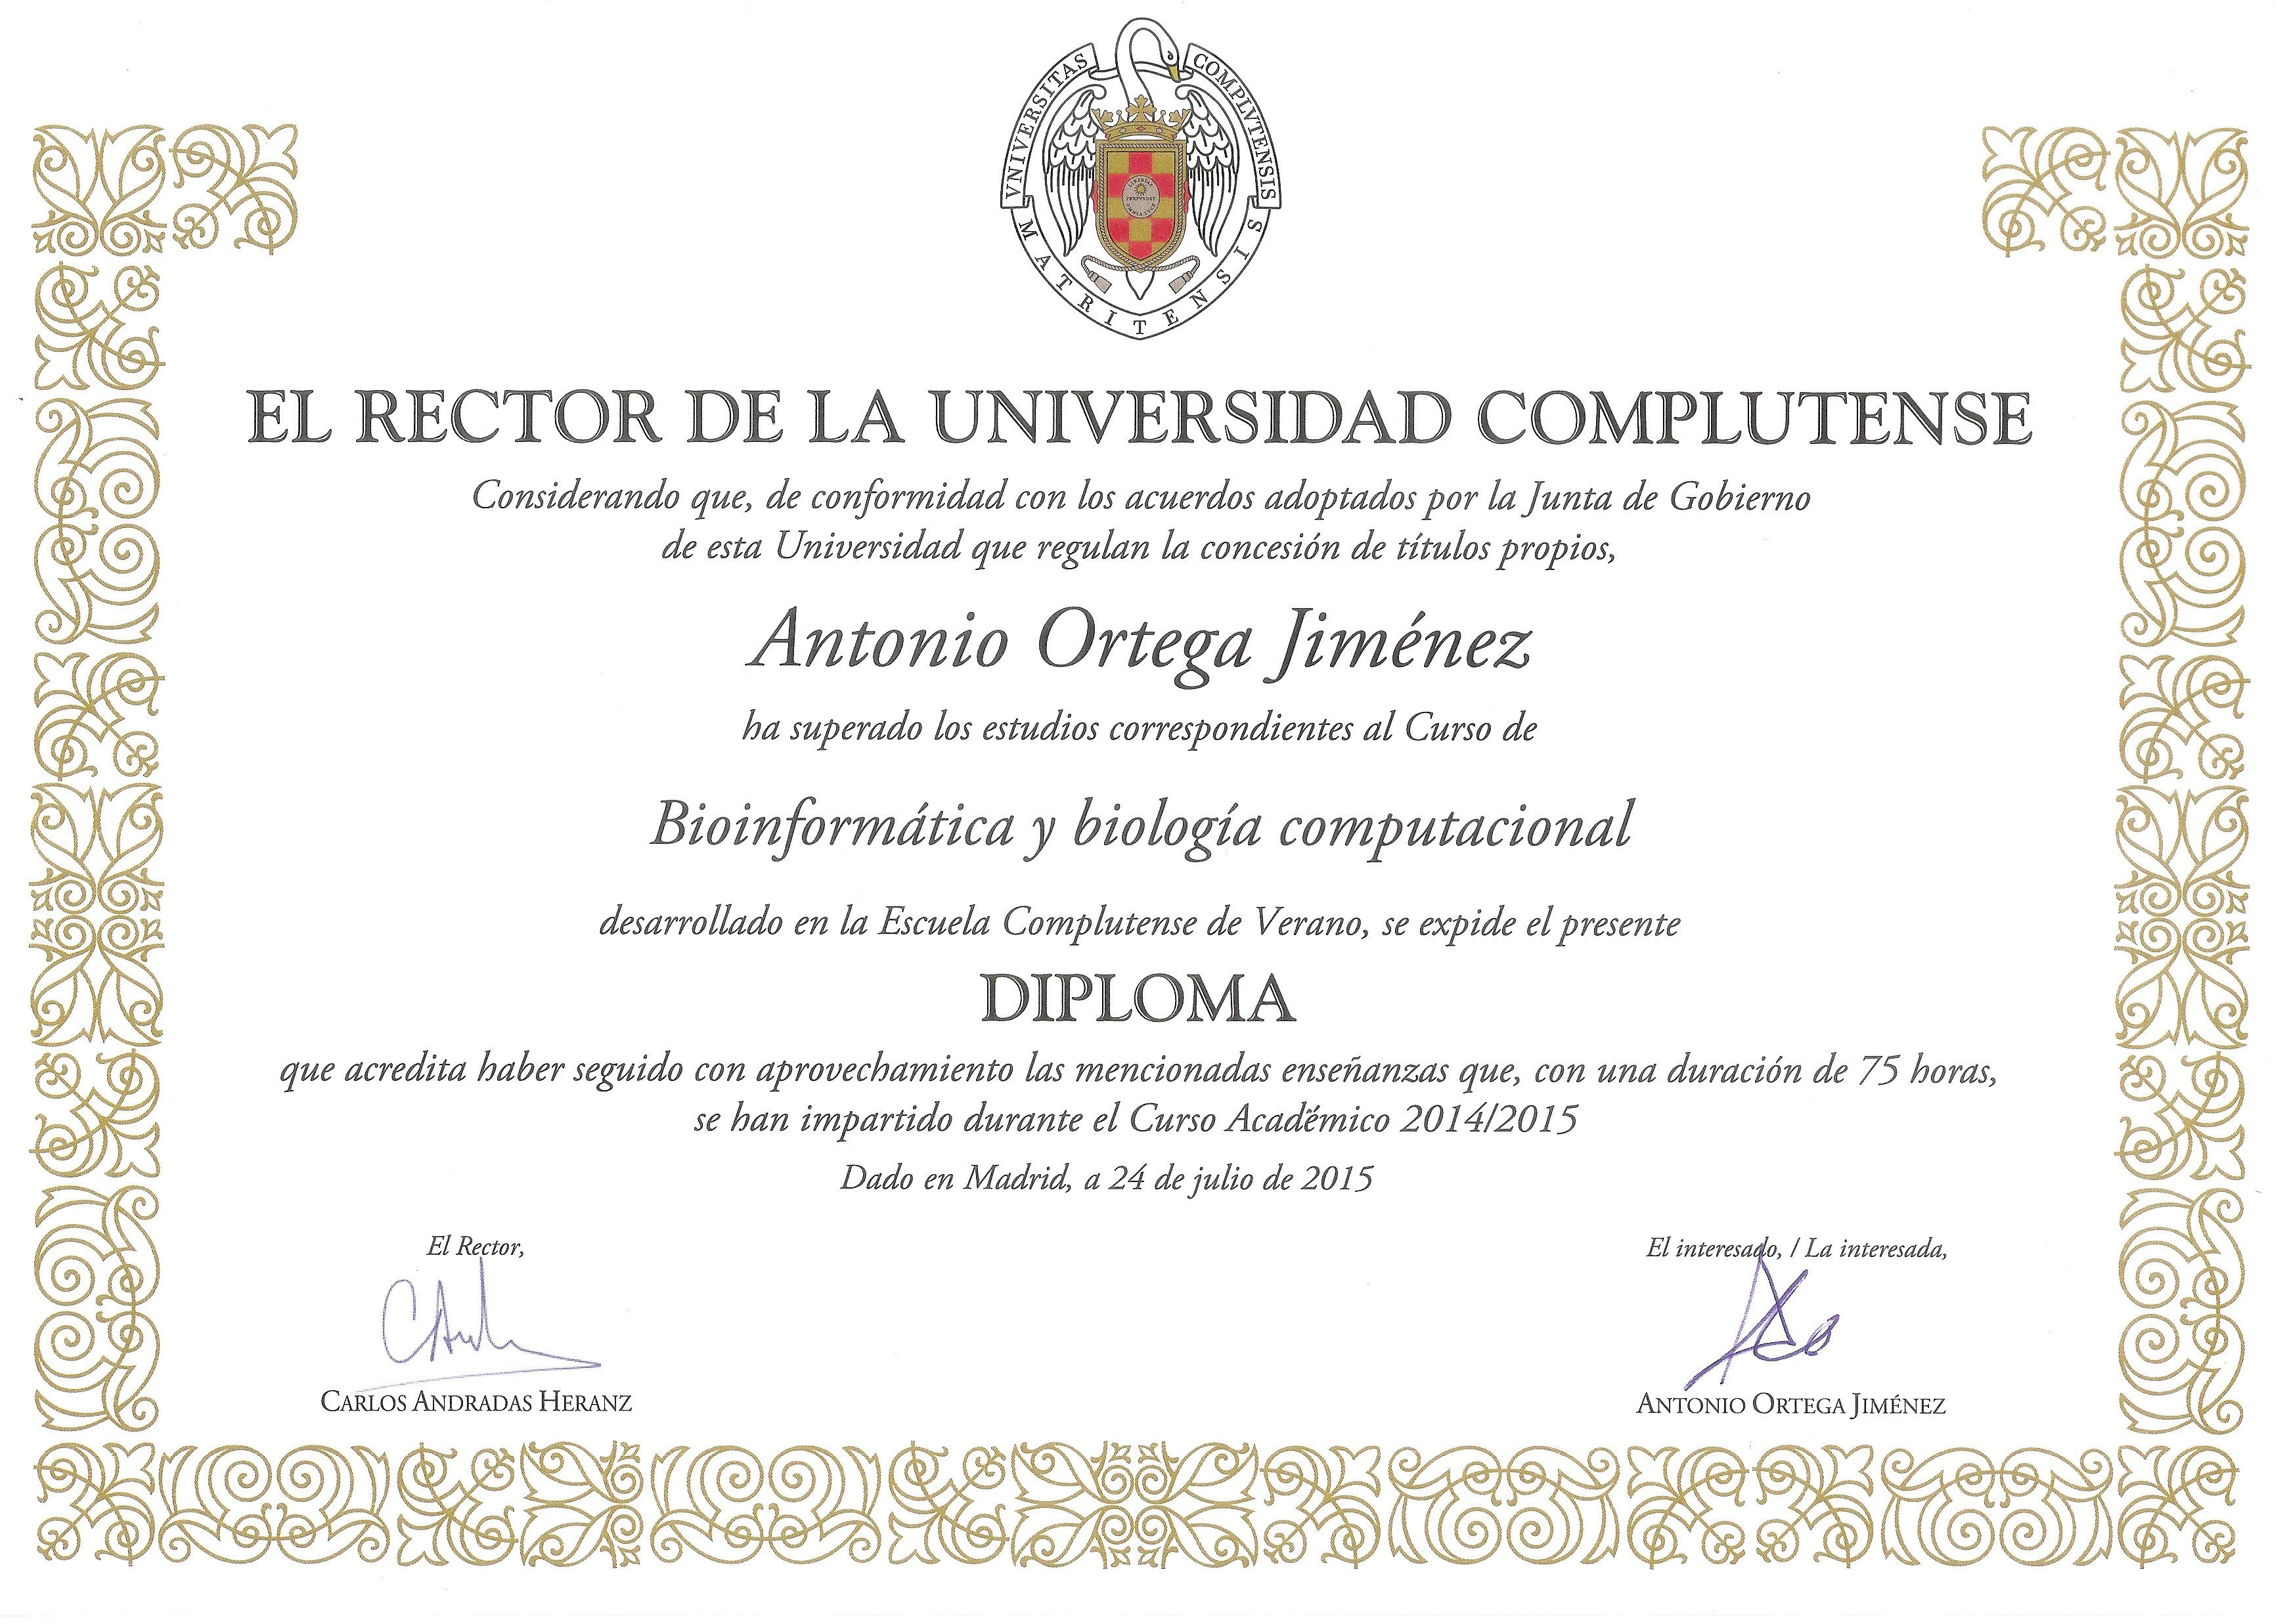
\includegraphics[scale=0.2]{append/bioinformatica2.jpg}
%\end{landscape}
%\restoregeometry
%\clearpage
%
%
%\newgeometry{margin=20pt, bottom=5pt}
%\hypertarget{ML-Coursera}{}
%\begin{landscape}
%\centering
%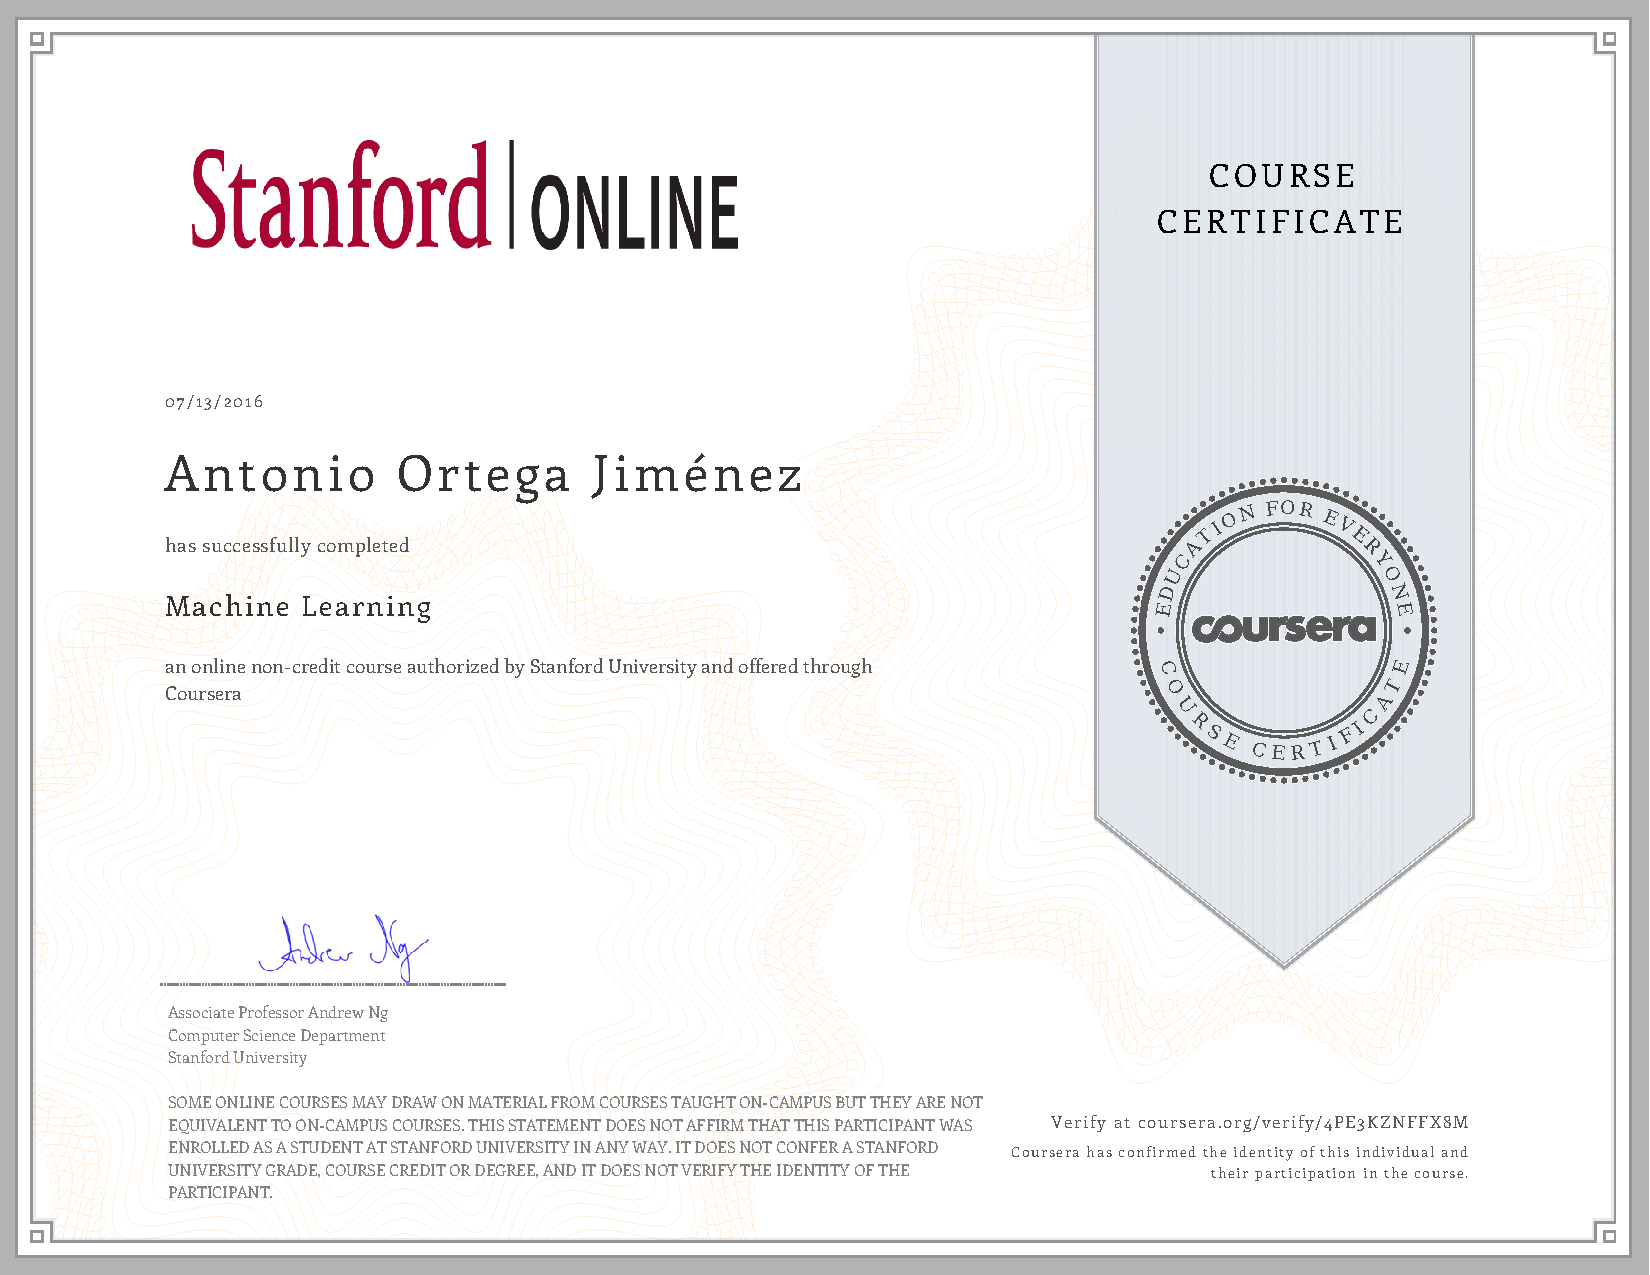
\includegraphics[width=\textwidth]{ML-Coursera.pdf}
%\end{landscape}
%\restoregeometry
%\clearpage
%
%
%%Expediente oficial en inglés
%\hypertarget{exp-en}{}
%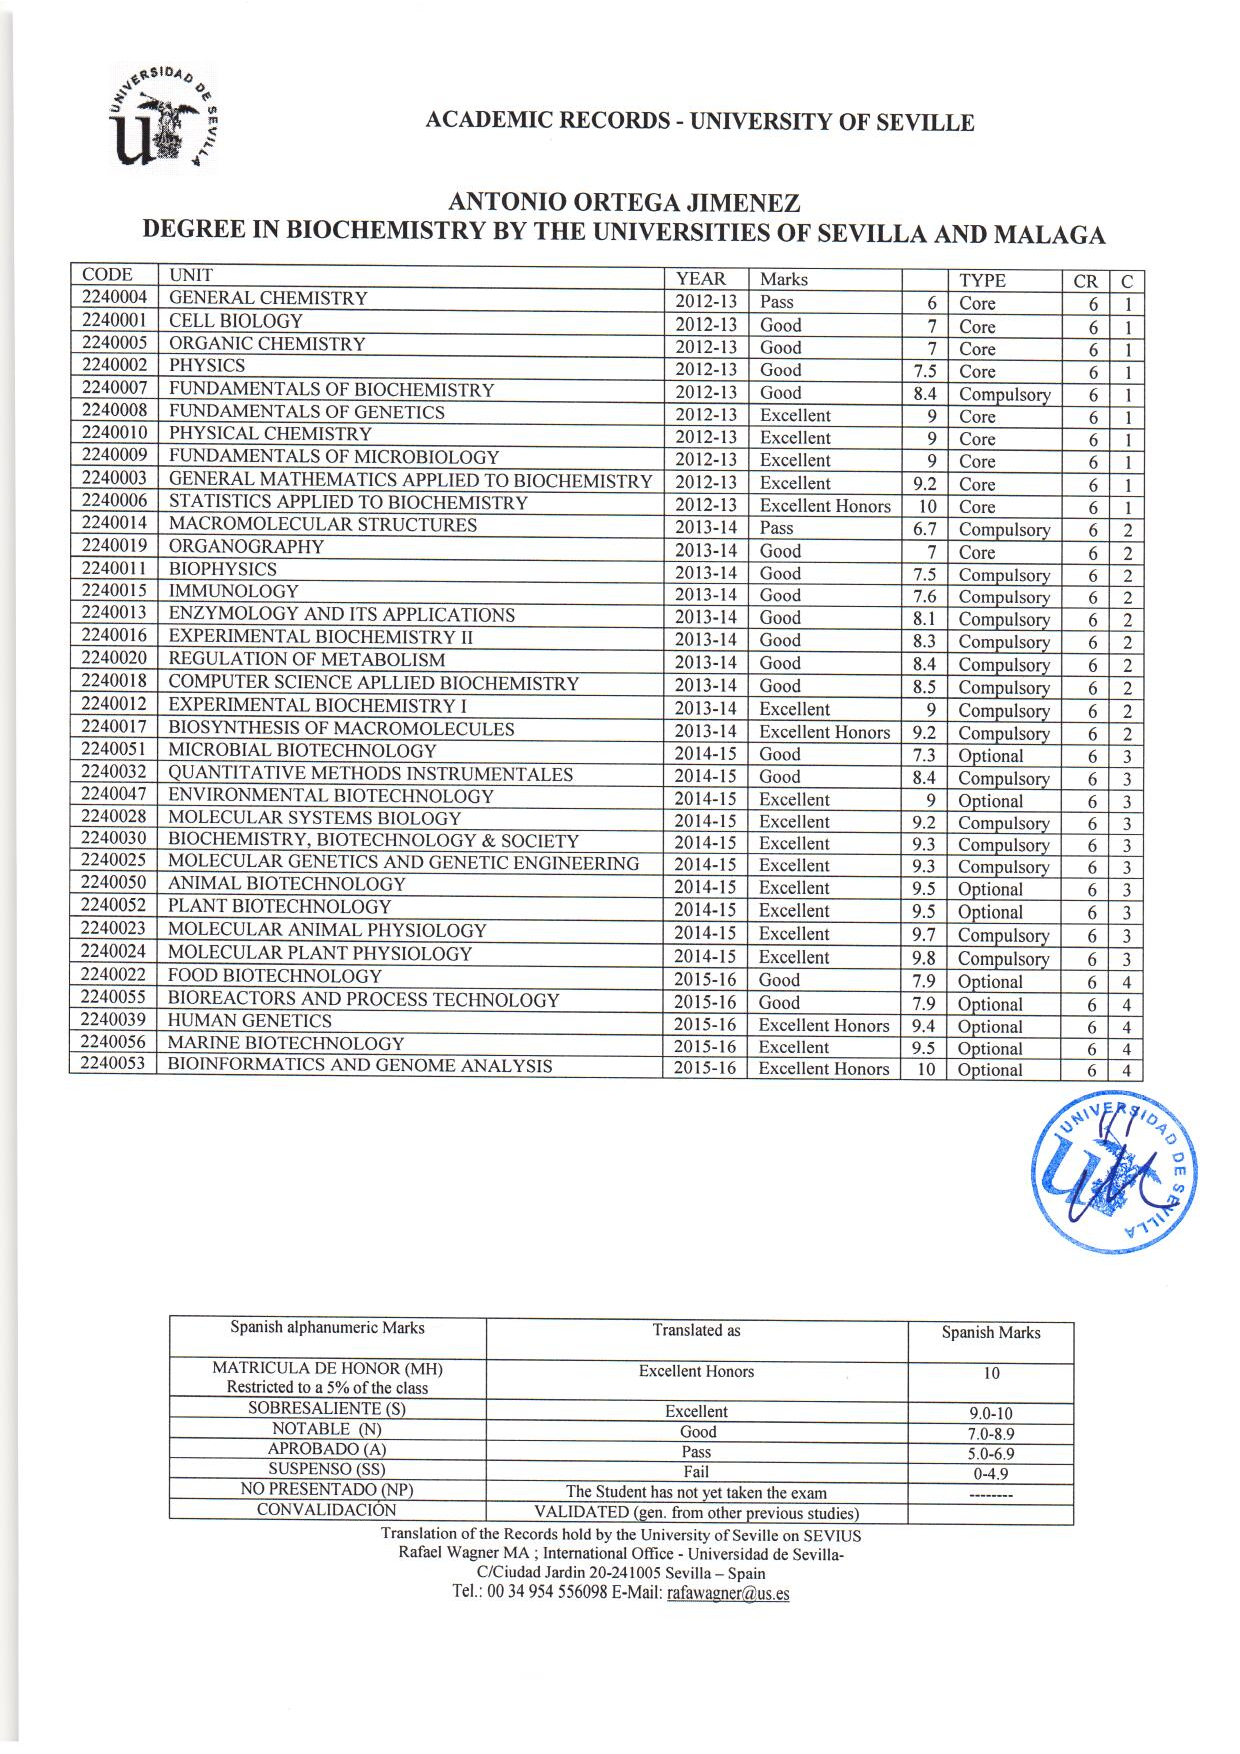
\includepdf[pages={1}]{Transcript-English.pdf}
%\clearpage
%
%
%\hypertarget{cae}{}
%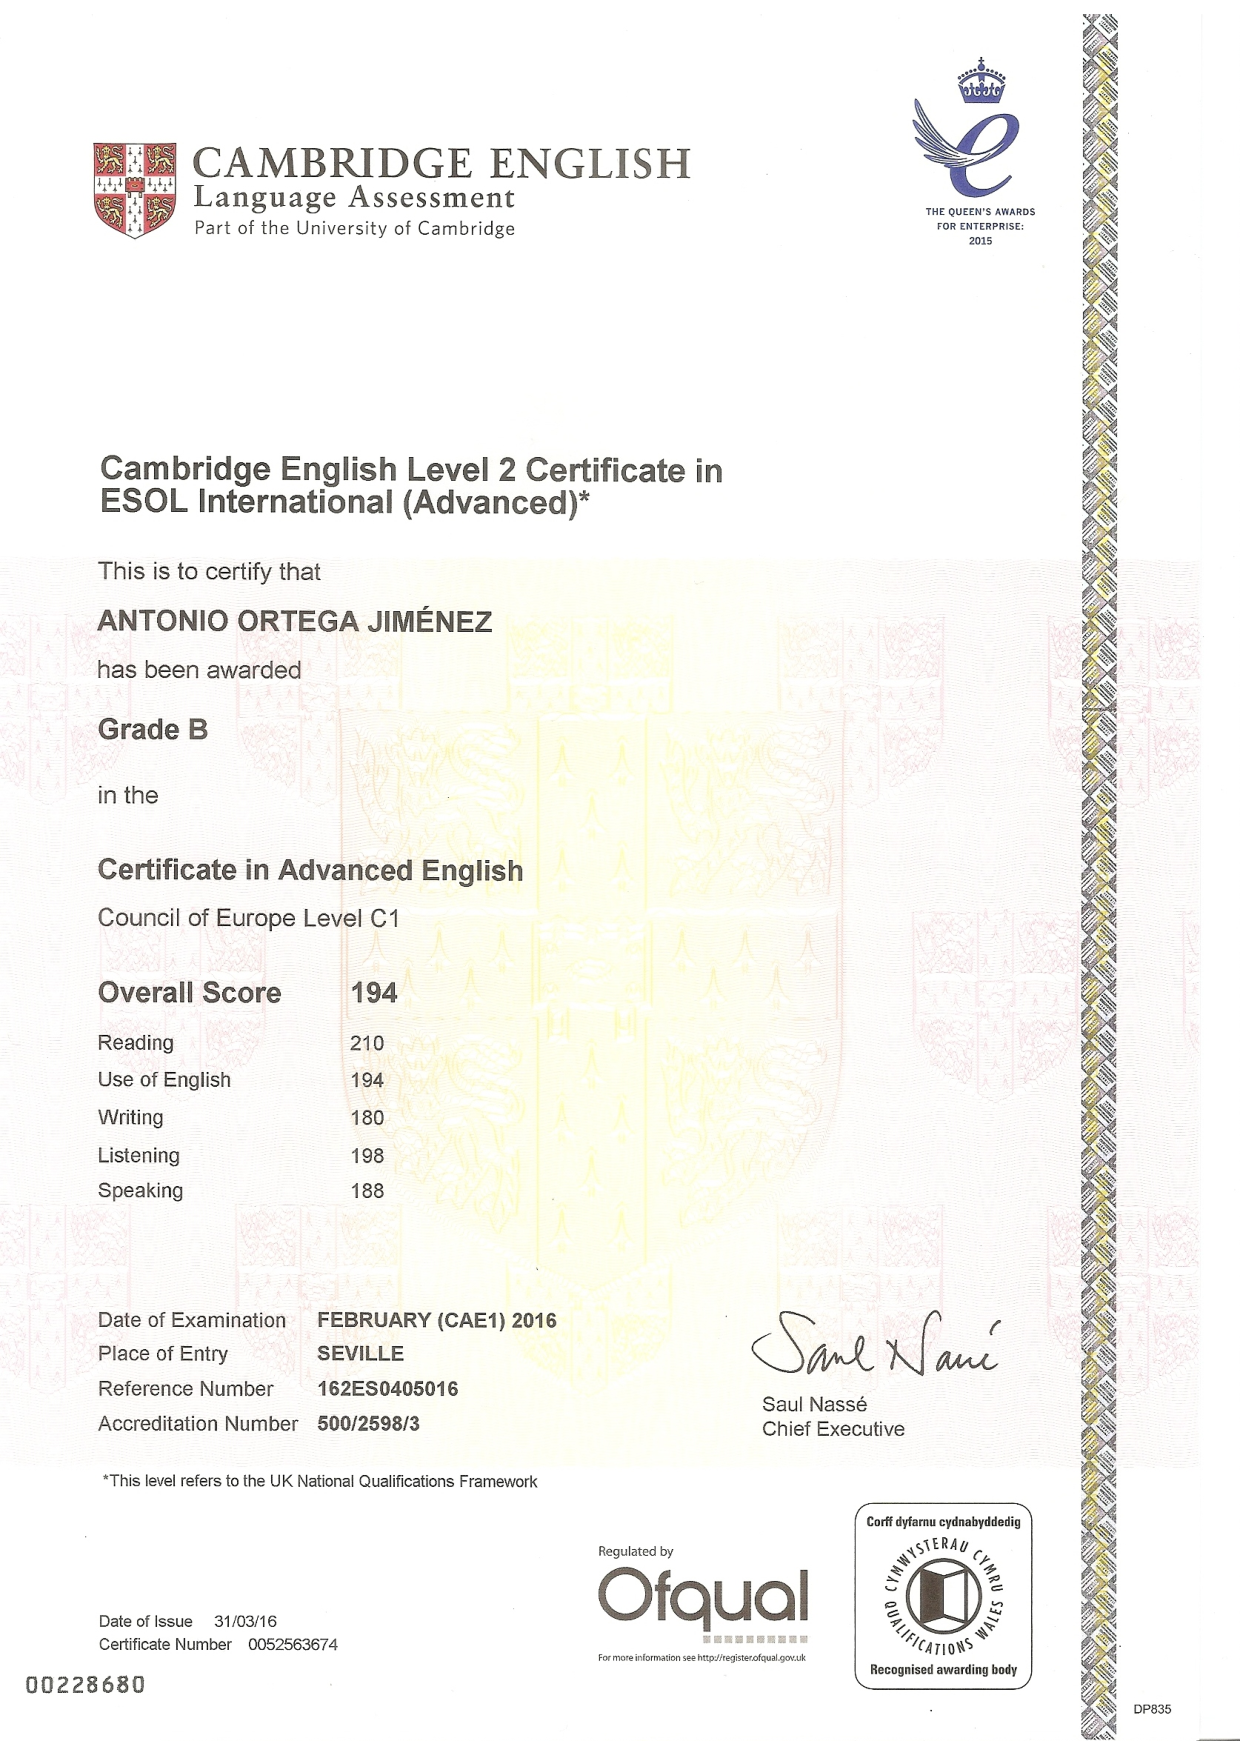
\includepdf{cae.pdf}
%\clearpage



%Certificado DELF
%\thispagestyle{empty}
%\begin{landscape}
%\begin{figure}
%\hspace{-2.5 cm}
%\includegraphics[scale=0.3]{append/delf.jpg}
%\end{figure}
%\end{landscape}
%\clearpage
\end{document}
